\documentclass[svgnames]{article}     % use "amsart" instead of "article" for AMSLaTeX format
%\geometry{landscape}                 % Activate for rotated page geometry

%\usepackage[parfill]{parskip}        % Activate to begin paragraphs with an empty line rather than an indent

\usepackage{graphicx}                 % Use pdf, png, jpg, or eps§ with pdflatex; use eps in DVI mode

%maths                                % TeX will automatically convert eps --> pdf in pdflatex
\usepackage{amssymb}
\usepackage{amsmath}
\usepackage{esint}
\usepackage[top = 0.3in, bottom = 0.3in]{geometry}

% Inverting Color of PDF
%\usepackage{xcolor}
%\pagecolor[rgb]{0.19,0.19,0.19}
%\color[rgb]{0.77,0.77,0.77}

%noindent
\setlength\parindent{0pt}

%pgfplots
\usepackage{pgfplots}

%images
%\graphicspath{{ }}                   % Activate to set a image directory

%tikz
\usepackage{pgfplots}
\pgfplotsset{compat=1.15}
\usepackage{comment}
\usetikzlibrary{arrows}
\usepackage[most]{tcolorbox}

%Figures
\usepackage{float}
\usepackage{caption}
\usepackage{lipsum}


\title{Degenerate Perturbation Theory}
\author{Deval Deliwala}
%\date{}                              % Activate to display a given date or no date

\begin{document}
\maketitle
%\section{}
%\subsection{}
%\tableofcontents                     % Activate to display a table of contents

If the unperturbed states are degenerate -- that is, if the distinct states
$\psi_a^{0}$ and $\psi_b^{0}$ share the same energy, then ordinary perturbation
theory fails. We derived the equations for the first-order correction to the
wave function,

\[
  \psi_n^{1} = \sum_{m\neq n}^{} \frac{\langle \psi_m^{0} | H' | \psi_n^{0}
\rangle}{E_n^{0} - E_m^{0}} \psi_m^{0} ,
\] \vspace{3px}

and the second-order correction to the energy, 

\[
E_n^2 = \sum_{m\neq n}^{} \frac{| \langle \psi_m^{0} | H' | \psi_n^{0}
\rangle|^2}{E_n^{0} - E_m^{0}}.
\] \vspace{3px}

Of course, if calculating $\psi_a^{1}$ or $E_a^{2}$, these equations blow up.
In the degenerate case, thus, there is no reason to trust even the
\textit{first} order correction to the energy. Almost all applications of
perturbation theory involves degeneracy. 

\section{Two-Fold Degeneracy}

Suppose we have two orthonormal solutions to the Schr\"odinger equation that
share the same energy eigenvalue, 

\begin{align}\label{ortho}
H^{0} \psi_a^{0} = E^{0} \psi_a^{0}, \quad H^{0} \psi_b^{0} = E^{0} \psi_b^{0},
\quad \langle \psi_a^{0} | \psi_b^{0} \rangle = 0,
\end{align} \vspace{3px}

with $\psi_a^{0}$ and $\psi_b^{0}$ being normalized. Any linear combination of
these states

\[
\psi^{0} = \alpha \psi_a^{0} + \beta \psi_b^{0}
\] \vspace{3px}

is also an eigenstate of $H^{0}$, with the same eigenvalue: 

\[
H^{0}\psi^{0} = E^{0} \psi^{0}. 
\] \vspace{3px}


Perturbation ($H'$ ), however, breaks (or ``lifts") the degeneracy. As we
increase $\lambda$ from 0 to 1, (unperturbed to perturbed), the common
unperturbed energy $E^{0}$ splits into two. 

\begin{figure}[H]
  \centering
    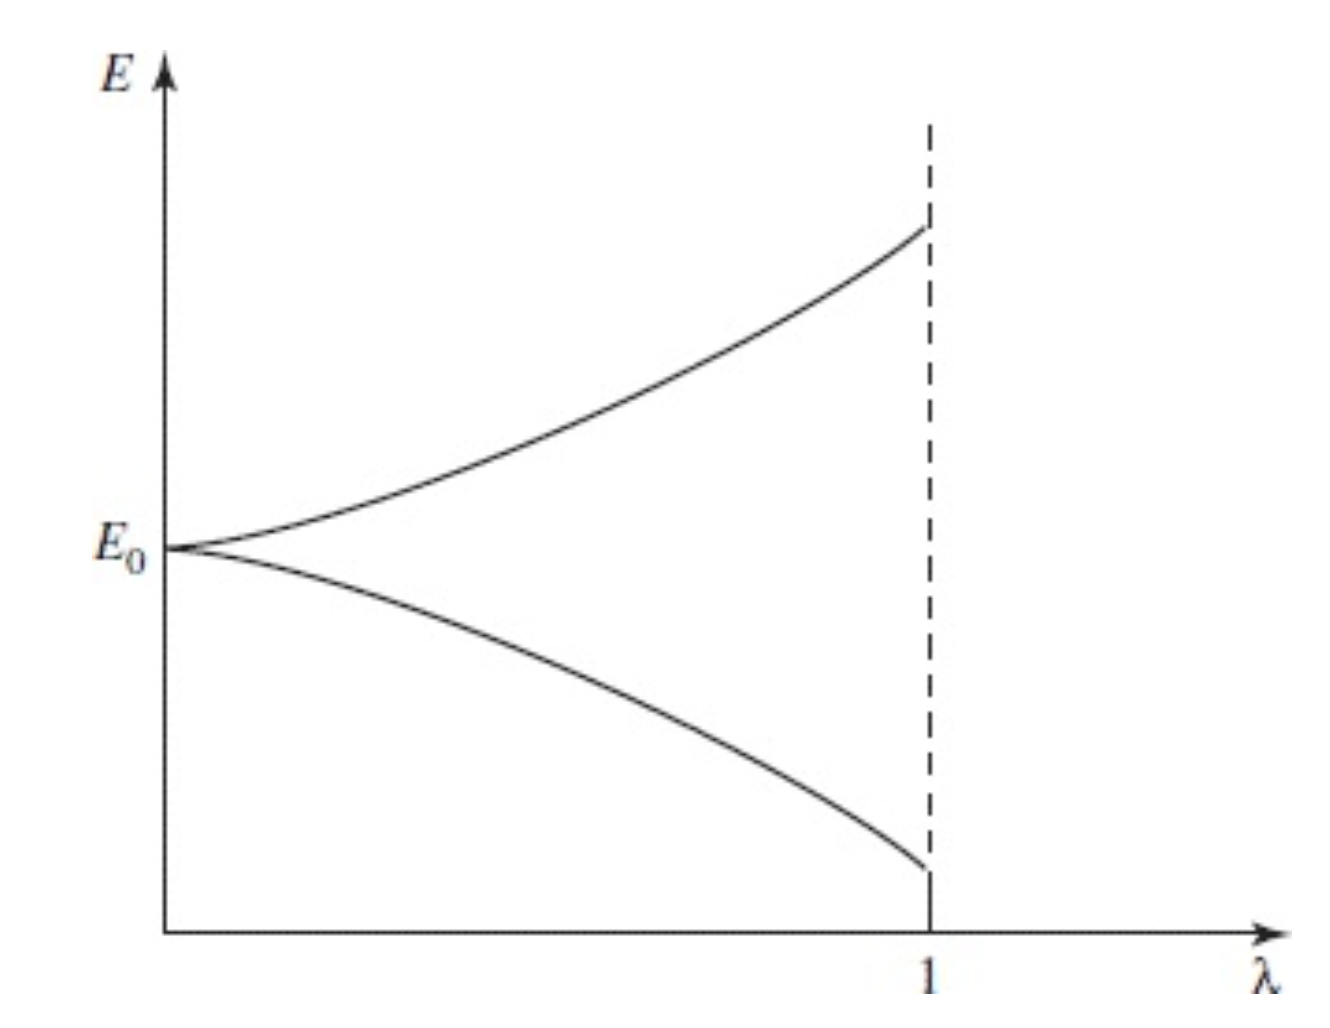
\includegraphics[width = 8cm]{screenshot.png}
\end{figure}


Going in the other direction, when we ``turn off" the perturbation, the
\textit{upper} state reduces down to one linear combination of $\psi_a^{0}$ and
$\psi_b^{0}$, and the \textit{lower} state reduces to some orthogonal linear
combination, but we don't know beforehand what these \textit{good} linear
combinations are. For this reason we can't evaluate the first-order energy
correction either -- we don't know what unperturbed states to use. 
\\
Put simply, because the original states were degenerate, it’s unclear which
combination of those degenerate states we should use to represent the ``new"
states after the perturbation is applied.
\\
The \textit{good} states are defined as the limit of the true eigenstates as
the perturbation is switched off ($\lambda \rightarrow 0$), but realistically,
if you \textit{knew} the exact eigenstates, you wouldn't need perturbation
theory, so what do we do? 

Let's first write the ``good" unperturbed states in a generic form, 

\begin{align}\label{base}
\psi^{0} = \alpha \psi_a^{0} + \beta \psi_b^{0}
\end{align} \vspace{3px}

keeping $\alpha$ and $\beta$ adjustable. We want to solve the Schr\"odinger
equation 

\begin{align}\label{hami}
H\psi = E\psi
\end{align} \vspace{3px}

with $H = H^{0} + \lambda H'$ and 

\[
E = E^{0} + \lambda E^{1} + \lambda ^2 E^2 + \cdots, \quad \psi = \psi^{0}
+ \lambda \psi^{1} + \lambda^2 \psi^2 + \cdots.
\] \vspace{3px}

Plugging into Equation \ref{hami}, and collecting like powers of $\lambda$ like
before, we get 

\[
H^{0}\psi^{0} + \lambda\left(H'\psi^{0} + H^{0}\psi^{1}\right) + \cdots
= E^{0}\psi^{0} + \lambda \left( E^{1}\psi^{0} + E^{0}\psi^{1} \right)
+ \cdots,  
\] \vspace{3px}

Cancelling out $H^{0}\psi^{0} = E^{0}\psi^{0}$, to order $\lambda^1$, we get 

\begin{align} \label{}
  H^0\psi^{1} + H'\psi^{0} = E^{0} \psi^{1} + E^{1}\psi^{0}. 
\end{align}\vspace{3px}


Now we take the inner product with $\hat{\psi_a^{0}}$, 

\[
\left\langle \psi_a^{0}| H^{0} \psi^{1} \right\rangle + \left\langle \psi_a^{0} | H' \psi^{0}
\right\rangle + E^{0} \left\langle \psi_a^{1} | \psi^{1} \right\rangle + E^{1}
\left\langle
\psi_a^{0}|\psi^{0} \right\rangle. 
\] \vspace{3px}


And again, since $H^{0}$ is hermitian, the first term on the left cancels the
first term on the right. Plugging in our generic ``good" unperturbed state
(Equation \ref{base}) and exploiting orthonormality (Equation \ref{ortho}), we
obtain 

\[
\alpha \left\langle \psi_a^{0} | H' | \psi_a^{0} \right\rangle + \beta \left\langle
\psi_a^{0} | H' | \psi_b^{0} \right\rangle = \alpha E^{1}
\] \vspace{3px}

or, more compactly, 

\begin{align} \label{w}
  \alpha W_{aa} + \beta W_{ab} = \alpha E^{1},
\end{align}\vspace{3px}


where 

\begin{align} \label{wdef}
  W_{ij} \equiv \left\langle \psi_i^{0} | H' | \psi_j^{0} \right\rangle. 
\end{align}\vspace{3px}

The $W$s are known -- they are just the matrix elements of $H'$ with respect to
the unperturbed wave functions $\psi_a^{0}$ and $\psi_b^{0}$. Similarly, taking the inner product with $\psi_b^{0}$ yields 

\begin{align} \label{w_2}
  \alpha W_{ba} + \beta W_{bb} = \beta E^{1}    
\end{align}\vspace{3px}

In matrix form, Equations \ref{w} and \ref{w_2} become

\begin{align} \label{weq}
  \begin{pmatrix}
    W_{aa} & W_{ab} \\ W_{ba} & W_{bb} 
  \end{pmatrix} \begin{pmatrix}
    \alpha \\ \beta
  \end{pmatrix} = E^{1} \begin{pmatrix}
    \alpha \\ \beta
  \end{pmatrix} . 
\end{align}\vspace{3px}


Therefore, $W$'s eigenvalues give the first order energy correction $E^{1}$,
and the corresponding eigenvectors tell us the coefficients $\alpha$ and
$\beta$ that give us the ``good" states. Solving for the eigenvalues yields 

\vspace{3px}
\begin{tcolorbox}[colback = blue!5!white, colframe = blue!50!black, title
  = First-order energy eigenvalues]

  \begin{align} \label{}
    E_\pm^{1} = \frac{1}{2} \left[ W_{aa} + W_{bb} \pm \sqrt{(W_{aa}
    - W_{bb})^2 + 4|W_{ab}|^2}\right].
  \end{align}\vspace{3px}

\end{tcolorbox}
\vspace{3px}
This is the fundamental result of degenerate perturbation theory. The two roots
correspond to the two split perturbed energies. 

If it happens that $W_{ab} = 0$, then the two eigenvectors are 

 \[
\begin{pmatrix}
  1 \\ 0
\end{pmatrix} \text{ and } \begin{pmatrix}
  0 \\ 1
\end{pmatrix} 
\] \vspace{3px}

and their energies, 

\[
  E_+^{1} = W_{aa} = \left\langle \psi_a^{0} | H' | \psi_a^{0} \right\rangle,
  \quad E_-^{1} = W_{bb} = \left\langle \psi_b^{0} | H' | \psi_b^{0}
    \right\rangle
\] \vspace{3px}

are precisely what we would have obtained via \textit{non}degenerate
perturbation theory. 

\section{``Good" States} 

I provide a theorem that allows one to \textit{guess} ``good" states. This
allows us to go ahead and just use ordinary \textit{non}degenerate perturbation
theory. \\

\noindent 
\textbf{Theorem}: Let $A$ be a hermitian operator that commutes with $H^{0}$
and $H'$. If $\psi_a^{0}$ and $\psi_b^{0}$ (the degenerate eigenfunctions of
$H^{0}$ are also eigenfunctions of $A$, with distinct eigenvalues, 

\[
A\psi^{0} = \mu \psi_a^{0}, \quad A\psi_b^{0} = \nu \psi_b^{0}, \quad \mu \neq
\nu,
\] \vspace{3px}

\noindent 
then $\psi_a^{0}$ and $\psi_b^{0}$ are ``good" states to use in perturbation
theory. \\

\noindent \textbf{Proof:} Since $H(\lambda) = H^{0} + \lambda H'$ and $A$
commute, there exist simultaneous eigenstates  $\psi_\gamma(\lambda)$ where 

\[
H(\lambda) \psi_\gamma (\lambda) = E(\lambda) \psi_\gamma(\lambda) \; \text{
and } \; A \psi_\gamma (\lambda) = \gamma \psi_\gamma (\lambda).
\] \vspace{3px}

The fact the $A$ is hermitian means

\begin{align*}
  \langle \psi_a^{0} | A \psi_\gamma (\lambda) \rangle &= \langle A \psi_a^{0}
  | \psi_\gamma(\lambda) \rangle  \\[5px]
  \gamma \langle  \psi_a^{0} | \psi_\gamma
  (\lambda) \rangle &= \mu^* \langle \psi_a^{0} | \psi_\gamma(\lambda) \rangle
  \\[5px] 
  (\gamma - \mu) \langle \psi_a^{0} | \psi_\gamma(\lambda) \rangle &= 0 
\end{align*}


making use of the fact that $\mu$ is real. This holds true for any value of
$\lambda$ and taking the limit as $\lambda \rightarrow 0$, we have 

\[
\left\langle \psi_a^{0} | \psi_\gamma(0) \right\rangle = 0 \quad \text{unless}
\quad \gamma = \mu,
\] \vspace{3px}

\noindent 
and similarly, 

\[
\left\langle \psi_b^{0} | \psi_\gamma (0) \right\rangle = 0 \quad \text{unless} \quad
  \gamma = \nu.
\] \vspace{3px}

Now the good states are linear combinations of $\psi_a^{0}$ and $\psi_b^{0}$
: $\psi_\gamma(0) = \alpha \psi_a^{0} + \beta \psi_b^{0}$. From above it follows
that either $\gamma = \mu$, in which case $\beta = \langle \psi_b^{0}
| \psi_\gamma(0) \rangle = 0$, and the  good state is simply $\psi_a^{0}$, or
$\gamma = \nu$ and the good state is $\psi_b^{0}$. 
\\

Once we identify the ``good" states by solving Equation \ref{weq},  we can use
these ``good" states as our unperturbed states and apply ordinary
non-degenerate perturbation theory. In most cases, the operator $A$ is
suggested by symmetry, as symmetries are associated with operators commuting
with the Hamiltonian -- precisely what we need. \\ 



Moral of the story -- If you are faced with degenerate states, look for
a hermitian operator $A$ that commutes with $H^{0}$ and $H'$. Pick you
unperturbed states as ones that are simultaneously eigenfunctions of $H^{0}$
and $A$ (with \textit{distinct} eigenvalues). Then use ordinary
\textit{non}degenerate perturbation theory. 

\section{Higher-order Degeneracy}

In the case of an $n$-fold degeneracy, we look for eigenvalues of the $n \times
n$ matrix 

\begin{align} \label{}
  W_{ij} = \left\langle \psi_i^{0} | H' | \psi_j^{0}\right\rangle.
\end{align}\vspace{3px}


For three fold degeneracy, (with degenerate states $\psi_a^{0}, \psi_b^{0},
\psi_c^{0}$), the first order corrections to the energies $E^{1}$ are the
eigenvalues of $W$, determined by solving 

\begin{align} \label{}
  \begin{pmatrix}
    W_{aa} & W_{ab} & W_{ac} \\ 
    W_{ba} & W_{bb} & W_{bc} \\ 
    W_{ca} & W_{cb} & W_{cc} 
  \end{pmatrix} \begin{pmatrix}
    \alpha \\ \beta \\ \gamma
  \end{pmatrix}  = E^{1} \begin{pmatrix}
    \alpha \\ \beta \\ \gamma
  \end{pmatrix} 
\end{align}\vspace{3px}

\noindent 

and the good states are the corresponding eigenvectors 

\[
\psi^{0} = \alpha \psi_a^{0} + \beta \psi_b^{0} + \gamma \psi_c^{0}. 
\] \vspace{3px}


Again, if you can find an operator $A$ that commutes with $H^{0}$ and $H'$, and
use the simultaneous eigenfunctions of $A$ and $H^{0}$, then the $W$ matrix
will \textit{automatically be diagonal}, and you won't have to calculate any
off-diagonal entries of $W$ or solve the characteristic equation. 
\end{document}

